\PassOptionsToPackage{unicode=true}{hyperref} % options for packages loaded elsewhere
\PassOptionsToPackage{hyphens}{url}
\PassOptionsToPackage{dvipsnames,svgnames*,x11names*}{xcolor}
%
\documentclass[ignorenonframetext,]{beamer}
\usepackage{pgfpages}
\setbeamertemplate{caption}[numbered]
\setbeamertemplate{caption label separator}{: }
\setbeamercolor{caption name}{fg=normal text.fg}
\beamertemplatenavigationsymbolsempty
% Prevent slide breaks in the middle of a paragraph:
\widowpenalties 1 10000
\raggedbottom
\setbeamertemplate{part page}{
\centering
\begin{beamercolorbox}[sep=16pt,center]{part title}
  \usebeamerfont{part title}\insertpart\par
\end{beamercolorbox}
}
\setbeamertemplate{section page}{
\centering
\begin{beamercolorbox}[sep=12pt,center]{part title}
  \usebeamerfont{section title}\insertsection\par
\end{beamercolorbox}
}
\setbeamertemplate{subsection page}{
\centering
\begin{beamercolorbox}[sep=8pt,center]{part title}
  \usebeamerfont{subsection title}\insertsubsection\par
\end{beamercolorbox}
}
\AtBeginPart{
  \frame{\partpage}
}
\AtBeginSection{
  \ifbibliography
  \else
    \frame{\sectionpage}
  \fi
}
\AtBeginSubsection{
  \frame{\subsectionpage}
}
\usepackage{lmodern}
\usepackage{amssymb,amsmath}
\usepackage{ifxetex,ifluatex}
\usepackage{fixltx2e} % provides \textsubscript
\ifnum 0\ifxetex 1\fi\ifluatex 1\fi=0 % if pdftex
  \usepackage[T1]{fontenc}
  \usepackage[utf8]{inputenc}
  \usepackage{textcomp} % provides euro and other symbols
\else % if luatex or xelatex
  \usepackage{unicode-math}
  \defaultfontfeatures{Ligatures=TeX,Scale=MatchLowercase}
\fi
% use upquote if available, for straight quotes in verbatim environments
\IfFileExists{upquote.sty}{\usepackage{upquote}}{}
% use microtype if available
\IfFileExists{microtype.sty}{%
\usepackage[]{microtype}
\UseMicrotypeSet[protrusion]{basicmath} % disable protrusion for tt fonts
}{}
\IfFileExists{parskip.sty}{%
\usepackage{parskip}
}{% else
\setlength{\parindent}{0pt}
\setlength{\parskip}{6pt plus 2pt minus 1pt}
}
\usepackage{xcolor}
\usepackage{hyperref}
\hypersetup{
            pdftitle={NEJM Statistical Guidelines for Authors},
            pdfauthor={Dave Harrington},
            colorlinks=true,
            linkcolor=darkblue,
            filecolor=Maroon,
            citecolor=darkblue,
            urlcolor=darkblue,
            breaklinks=true}
\urlstyle{same}  % don't use monospace font for urls
\newif\ifbibliography
\usepackage{longtable,booktabs}
\usepackage{caption}
% These lines are needed to make table captions work with longtable:
\makeatletter
\def\fnum@table{\tablename~\thetable}
\makeatother
\usepackage{graphicx,grffile}
\makeatletter
\def\maxwidth{\ifdim\Gin@nat@width>\linewidth\linewidth\else\Gin@nat@width\fi}
\def\maxheight{\ifdim\Gin@nat@height>\textheight\textheight\else\Gin@nat@height\fi}
\makeatother
% Scale images if necessary, so that they will not overflow the page
% margins by default, and it is still possible to overwrite the defaults
% using explicit options in \includegraphics[width, height, ...]{}
\setkeys{Gin}{width=\maxwidth,height=\maxheight,keepaspectratio}
\setlength{\emergencystretch}{3em}  % prevent overfull lines
\providecommand{\tightlist}{%
  \setlength{\itemsep}{0pt}\setlength{\parskip}{0pt}}
\setcounter{secnumdepth}{0}

% set default figure placement to htbp
\makeatletter
\def\fps@figure{htbp}
\makeatother


\usepackage{amsmath,verbatim}

\usepackage{fancyvrb}
\usepackage{manfnt}
\usepackage[normalem]{ulem}

%\usepackage[colorlinks=true]{hyperref}

\mode<presentation>{\usetheme{Malmoe}}

%\synctex=1

\setbeamertemplate{headline}{}


\setbeamerfont{footline}{size=\scriptsize}
\setbeamerfont{frametitle}{shape=\scshape}
\setbeamertemplate{itemize items}[circle]
\setbeamercovered{transparent}

\setbeamertemplate{navigation symbols}{}
\setbeamertemplate{footline}[frame number]{} 


\definecolor{forest}{rgb}{0, .5, 0}
\definecolor{brick}{rgb}{.5, 0, 0}
\definecolor{darkgreen}{rgb}{0, .5, 0}
\definecolor{darkred}{rgb}{.7, .15, .15}
\definecolor{darkblue}{rgb}{0, 0, .5}
\definecolor{Green}{rgb}{0.2,1,0.2}


\newcommand{\R}{\textsf{R}}
\newcommand{\RStudio}{\textsl{R Studio}}


\usepackage[english]{babel}
%\usepackage{palatino}
%\usepackage[T1]{fontenc}
\usepackage[utf8]{inputenc}

% make all tt fonts bold to look more like Verbatim
\usepackage{lmodern}
\renewcommand\ttfamily{\usefont{T1}{lmtt}{m}{n}}

% Comment these out if you don't want a slide with just the
% part/section/subsection/subsubsection title:
\AtBeginPart{
  \let\insertpartnumber\relax
  \let\partname\relax
  \frame{\partpage}
}
\AtBeginSection{
  \let\insertsectionnumber\relax
 \let\sectionname\relax
 \frame{\sectionpage}
}
\AtBeginSubsection{
  \let\insertsubsectionnumber\relax
  \let\subsectionname\relax
  \frame{\subsectionpage}
}

\logo{
\includegraphics[width=.50\textwidth]{../figures/DFCI_DDS_Logo.png}\hspace*{.55\paperwidth}\vspace*{-.2in}}
\newcommand{\nologo}{\setbeamertemplate{logo}{}} % command to set the logo to nothing

\title{NEJM Statistical Guidelines for Authors}
\author{Dave Harrington}
\date{17 September 2019}

\begin{document}
\frame{\titlepage}

\begin{frame}{My coordinates}
\protect\hypertarget{my-coordinates}{}

\begin{itemize}
\item
  Department of Biostatistics, Harvard T.H. Chan School of Public Health
\item
  Department of Data Sciences, Dana-Farber Cancer Institute
\item
  Statistical Consultant, New England Journal of Medicine
\item
  Member, MSKCC Phase 3 DSMB
\item
  \href{mailto:davidharrington@g.harvard.edu}{\nolinkurl{davidharrington@g.harvard.edu}}
\end{itemize}

\end{frame}

\begin{frame}{Background}
\protect\hypertarget{background}{}

Revised author guidelines on statistical reporting posted on NEJM
website 1 July 2019

\url{https://www.nejm.org/author-center/new-manuscripts}

Goal: More consistency in both statistical reviews and articles

Editorial describing the guidelines published 18 July 2019

\begin{itemize}
\tightlist
\item
  N Engl J Med 2019; 381:285-286
\end{itemize}

Guidelines cover many aspects of statistical reporting

Editorial emphasized section on p-values

\end{frame}

\begin{frame}{Navigating NEJM}
\protect\hypertarget{navigating-nejm}{}

\centering

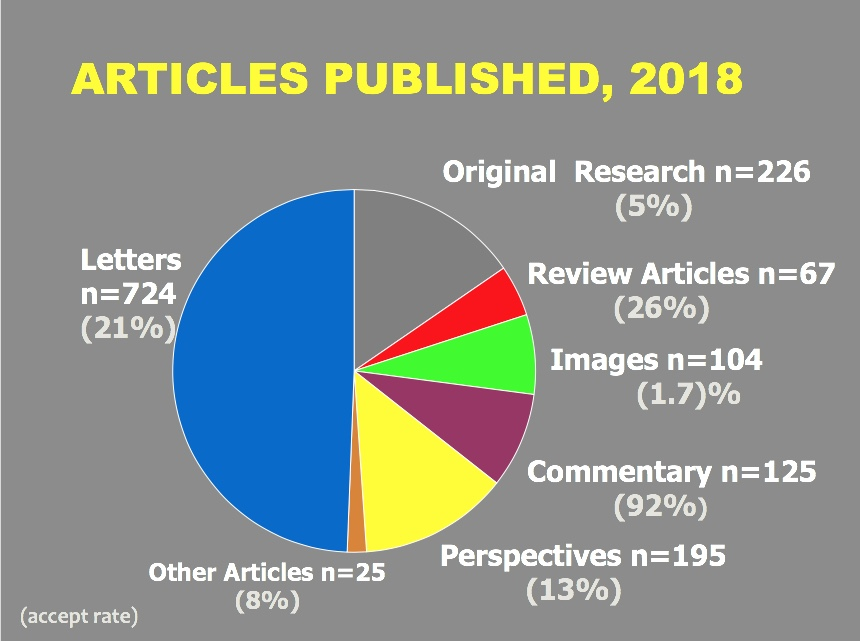
\includegraphics[width=1\textwidth,height=\textheight]{../figures/articles_published_2018.jpeg}

\end{frame}

\begin{frame}{Statistical Review at NEJM}
\protect\hypertarget{statistical-review-at-nejm}{}

Six paid statistical consultants (reviewers)

We meet weekly with the editors

Review all research articles that editors decide to move through the
system

\begin{itemize}
\tightlist
\item
  We see approximately 5\% of the 5,000 - 6000 submitted articles
\end{itemize}

Statistical reviewers

\begin{itemize}
\item
  Help set statistical `policy'
\item
  Work toward consistency in reviews
\end{itemize}

\end{frame}

\begin{frame}{Why did we fuss with \(p\)-values?}
\protect\hypertarget{why-did-we-fuss-with-p-values}{}

Many submitted manuscripts side-stepped the issue of multiplicity

\begin{itemize}
\item
  Possibly inflated type 1 error rates when comparing many endpoints to
  assess an intervention or an exposure
\item
  True in both randomized trials and observational studies
\item
  Becoming more prevalent in complex studies with many measurements
\end{itemize}

Particularly important in trials with negative primary outcomes

VITAL trial is a useful example

\end{frame}

\begin{frame}{VITAL: \underline{Vit}amin D and Omega-3
Tri\underline{al}}
\protect\hypertarget{vital-amin-d-and-omega-3-tri}{}

Manson JE, et al.~NEJM 2019; 380:23-32 (3 Jan 2019)

Factorial design, (Vit D vs placebo) \(\times\) (Omega-3 vs placebo)

25,871 participants randomized

\begin{itemize}
\tightlist
\item
  12,927 Vit D vs 12,944 placebo\\
\item
  12,933 n-3 vs 12,938 placebo
\end{itemize}

Primary endpoints: invasive cancer, composite cardiovascular outcome

\end{frame}

\begin{frame}{Omega-3 vs placebo comparison}
\protect\hypertarget{omega-3-vs-placebo-comparison}{}

2 co-primary endpoints: invasive cancer, composite CV outcome

\begin{itemize}
\tightlist
\item
  Both negative
\end{itemize}

22 secondary/exploratory outcomes

2 traditionally significant

\begin{itemize}
\tightlist
\item
  Total MI, total coronary heart disease (composite)
\end{itemize}

13 subgroups analyzed for possible treatment interactions

\begin{itemize}
\tightlist
\item
  No `significant' (\(p < 0.05\)) interactions
\end{itemize}

\end{frame}

\begin{frame}{`Black Box' warning in the protocol}
\protect\hypertarget{black-box-warning-in-the-protocol}{}

\begin{quote}

There was no control for multiple hypothesis testing, and no formal adjustment was made to the P values or confidence intervals. Thus, the results regarding exploratory end points and subgroups should be interpreted with caution. 

\end{quote}

What is the potential harm?

\begin{itemize}
\item
  None, if the \(p\)-value is a simple descriptor of a calculation
\item
  Considerably more, if a few significant comparisons are viewed as
  evidence for a treatment effect

  \begin{itemize}
  \tightlist
  \item
    Especially when the primary outcome is negative
  \end{itemize}
\end{itemize}

\end{frame}

\begin{frame}{P-values in medical literature}
\protect\hypertarget{p-values-in-medical-literature}{}

\(p < 0.05\) proposed by Fisher (1926) for single comparisons in
randomized experiments:

\begin{quote}

The value for which $P = 0.05$, or 1 in 20, is 1.96 or nearly 2; it is convenient to take this point as a limit in judging whether a deviation ought to be considered significant or not. 

\end{quote}

A \(p\)-value measures how much the observed data disagree with a
hypothesis of no treatment effect.

It is sometimes incorrectly interpreted as a measure of the
reproducibility of a trial

\begin{itemize}
\tightlist
\item
  or \(p < 0.05\) implies that the chance that the intervention works is
  at least 95\%
\end{itemize}

\end{frame}

\begin{frame}{Analogy with diagnostic testing}
\protect\hypertarget{analogy-with-diagnostic-testing}{}

In a hypothesis test

Power of the test is likelihood of detecting a true effect

\begin{itemize}
\tightlist
\item
  \textcolor{darkblue}{Sensitivity}
\end{itemize}

Significance level of a test is the chance of test being positive when
effect is null

\begin{itemize}
\tightlist
\item
  It is the false positive rate, or
  \textcolor{darkblue}{1 - Specificity}
\end{itemize}

The positive predictive value of a hypothesis test is the chance the
intervention is effective when the test is statistically significant

\end{frame}

\begin{frame}{Prevalence affects false positive rate}
\protect\hypertarget{prevalence-affects-false-positive-rate}{}

Next slide shows a graph of
\textcolor{darkblue}{probability of a false positive} conclusion in
favor after a \textcolor{darkblue}{statistically significant} result,
based on

\begin{itemize}
\item
  Power of the study
\item
  Significance level threshold
\item
  \textcolor{forest}{Prior odds of a treatment effect}
\end{itemize}

\end{frame}

\begin{frame}{False positive probability, p-value, power (Nat. Human
Behavior, Jan 2018)}
\protect\hypertarget{false-positive-probability-p-value-power-nat.-human-behavior-jan-2018}{}

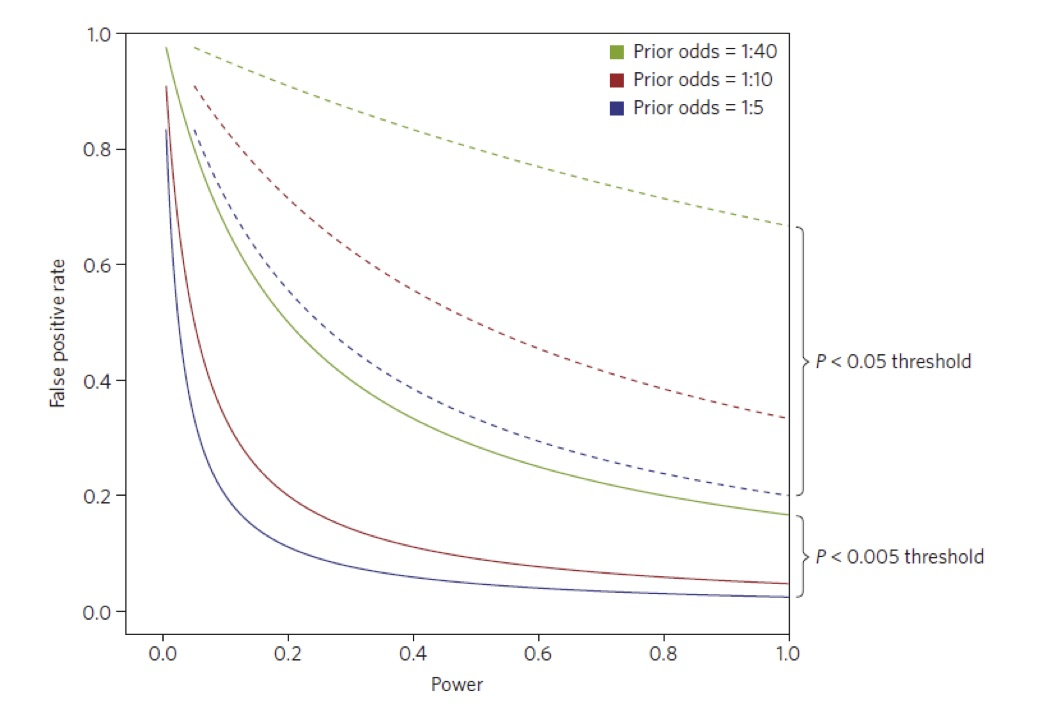
\includegraphics[width=1\textwidth,height=\textheight]{../figures/ppv_threshold.jpeg}

\end{frame}

\begin{frame}{What if the actual threshold for a `significant' result is
larger than 0.05?}
\protect\hypertarget{what-if-the-actual-threshold-for-a-significant-result-is-larger-than-0.05}{}

\begin{longtable}[]{@{}llll@{}}
\toprule
Alpha & Prior Odds & Prob Null & False Pos. Prob\tabularnewline
\midrule
\endhead
0.1 & 1:5 & 0.83 & 0.38\tabularnewline
0.1 & 1:10 & 0.91 & 0.56\tabularnewline
0.1 & 1:40 & 0.98 & 0.83\tabularnewline
0.25 & 1:5 & 0.83 & 0.61\tabularnewline
0.25 & 1:10 & 0.91 & 0.76\tabularnewline
0.25 & 1:40 & 0.98 & 0.93\tabularnewline
\bottomrule
\end{longtable}

False Pos. Prob = probability of incorrectly claiming alternative is
true, given data

Calculations assume power = 0.80

\end{frame}

\begin{frame}{The effect of multiplicity}
\protect\hypertarget{the-effect-of-multiplicity}{}

The more tests in a set of comparisons, the more likely it is that at
least one will be a false positive. \medskip

Suppose each test is done at level \(\alpha = 0.05\), and the endpoints
are independent.

\begin{longtable}[]{@{}cr@{}}
\toprule
\begin{minipage}[b]{0.34\columnwidth}\centering
Number of Comparisons\strut
\end{minipage} & \begin{minipage}[b]{0.39\columnwidth}\raggedleft
Overall Type I Error Prob.\strut
\end{minipage}\tabularnewline
\midrule
\endhead
\begin{minipage}[t]{0.34\columnwidth}\centering
1\strut
\end{minipage} & \begin{minipage}[t]{0.39\columnwidth}\raggedleft
0.05\strut
\end{minipage}\tabularnewline
\begin{minipage}[t]{0.34\columnwidth}\centering
2\strut
\end{minipage} & \begin{minipage}[t]{0.39\columnwidth}\raggedleft
0.10\strut
\end{minipage}\tabularnewline
\begin{minipage}[t]{0.34\columnwidth}\centering
3\strut
\end{minipage} & \begin{minipage}[t]{0.39\columnwidth}\raggedleft
0.14\strut
\end{minipage}\tabularnewline
\begin{minipage}[t]{0.34\columnwidth}\centering
5\strut
\end{minipage} & \begin{minipage}[t]{0.39\columnwidth}\raggedleft
0.23\strut
\end{minipage}\tabularnewline
\begin{minipage}[t]{0.34\columnwidth}\centering
10\strut
\end{minipage} & \begin{minipage}[t]{0.39\columnwidth}\raggedleft
0.40\strut
\end{minipage}\tabularnewline
\begin{minipage}[t]{0.34\columnwidth}\centering
20\strut
\end{minipage} & \begin{minipage}[t]{0.39\columnwidth}\raggedleft
0.64\strut
\end{minipage}\tabularnewline
\bottomrule
\end{longtable}

\end{frame}

\begin{frame}{Effect of increasing \(\alpha\)}
\protect\hypertarget{effect-of-increasing-alpha}{}

Prior odds = 1:10, power = 0.80

\begin{longtable}[]{@{}rr@{}}
\toprule
Alpha & False Pos. Prob.\tabularnewline
\midrule
\endhead
0.10 & 0.56\tabularnewline
0.15 & 0.65\tabularnewline
0.20 & 0.71\tabularnewline
0.25 & 0.76\tabularnewline
0.40 & 0.83\tabularnewline
0.60 & 0.88\tabularnewline
\bottomrule
\end{longtable}

False Pos. Prob. = probability of incorrectly claiming alternative is
true, given data

\end{frame}

\begin{frame}{Not just a theoretical issue}
\protect\hypertarget{not-just-a-theoretical-issue}{}

Between 2000 and 2010:

\begin{itemize}
\item
  1425 RCTs published in NEJM
\item
  Among these trials, 222/1425 negative primary outcomes
\item
  Among trials with negative primary outcomes, 121/222 ``positive''
  secondary outcomes or subgroup by treatment interactions

  \begin{itemize}
  \tightlist
  \item
    73 with a positive subgroup\\
  \item
    36 positive secondary outcome\\
  \item
    12 with `nearly positive' outcome
  \end{itemize}
\item
  Of 121 with a presumed signal

  \begin{itemize}
  \tightlist
  \item
    21 were replicated and showed positive primary outcome
  \end{itemize}
\end{itemize}

\end{frame}

\begin{frame}{Recommendations in the current guidelines}
\protect\hypertarget{recommendations-in-the-current-guidelines}{}

If a statistically sound method for multiple tests was specified in the
protocol or SAP, please follow it explicitly.

If there was no such plan

\begin{itemize}
\item
  Acknowledge the lack of a plan.
\item
  Report secondary outcomes using only point estimates of treatment
  effect and 95\% confidence intervals.
\item
  Specifically state that the confidence intervals have not been
  adjusted for multiplicity and cannot be used to support claims about
  treatment effects.
\end{itemize}

\end{frame}

\begin{frame}{Implications of the recommendations}
\protect\hypertarget{implications-of-the-recommendations}{}

Makes available all data on primary and secondary outcomes

\begin{itemize}
\item
  Without conclusions not likely to be reproducible
\item
  What did you see vs.~what did you learn?
\end{itemize}

Confidence intervals are more informative than \(p\)-values

Makes demands of our readers

Requires careful editing of manuscripts

Policy applies to observational studies as well as RCTs

A purely statistical perspective oversimplifies the treatment of
negative trials.

\begin{itemize}
\tightlist
\item
  See Pocock and Stone, NEJM 2016: ``The primary outcome fails \ldots''
\end{itemize}

\end{frame}

\begin{frame}{Shanafelt, et al.~NEJM 2019}
\protect\hypertarget{shanafelt-et-al.nejm-2019}{}

\begin{quote}

Patients 70 years of age or younger with previously untreated CLL were randomly assigned to receive ibrutinib plus rituximab or chemoimmunotherapy with fludarabine, cyclophosphamide, and rituximab.

The ibrutinib-based regimen led to prolonged progression-free and overall survival.

\end{quote}

Figure 2 from article on next slide

\end{frame}

\begin{frame}

\centering

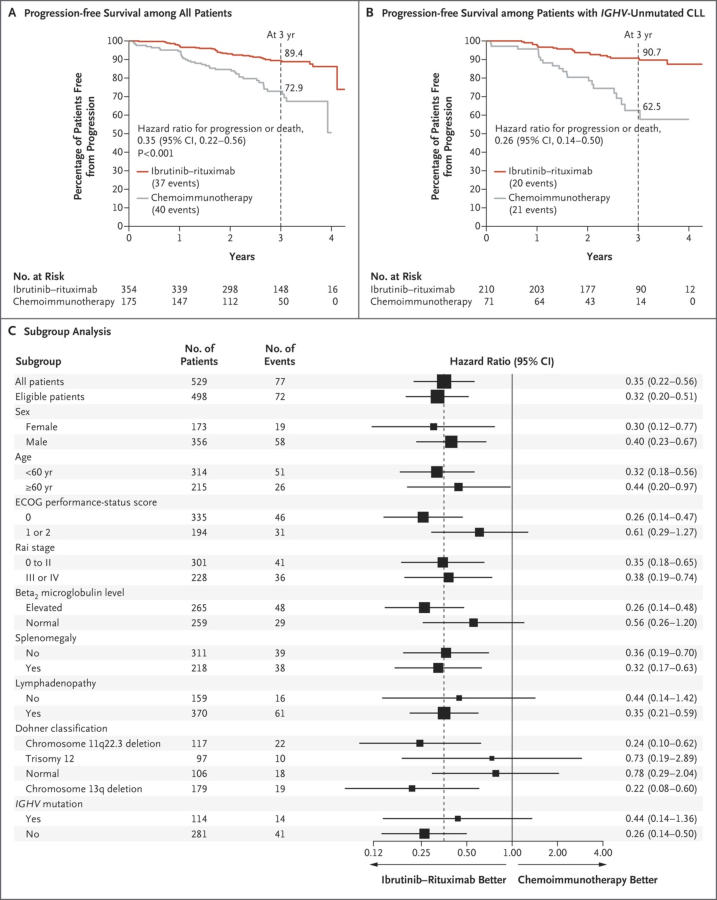
\includegraphics[width=0.6\textwidth,height=\textheight]{../figures/shanafelt_cll.pdf}

\end{frame}

\begin{frame}{The PFS curves}
\protect\hypertarget{the-pfs-curves}{}

\centering

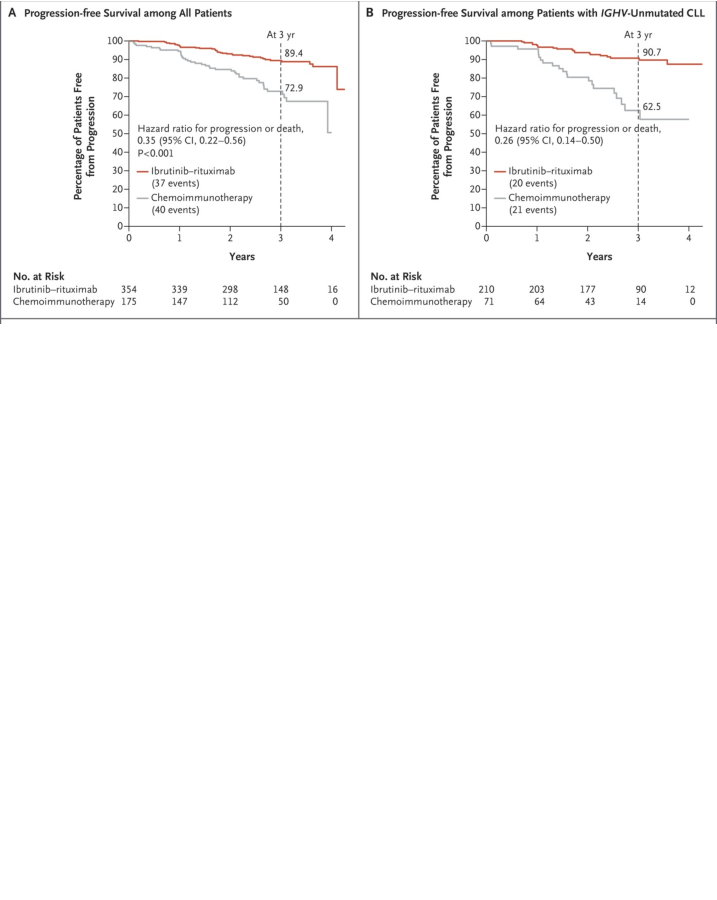
\includegraphics{../figures/shanafelt_curves.pdf}

\end{frame}

\begin{frame}{Subgroups}
\protect\hypertarget{subgroups}{}

\centering

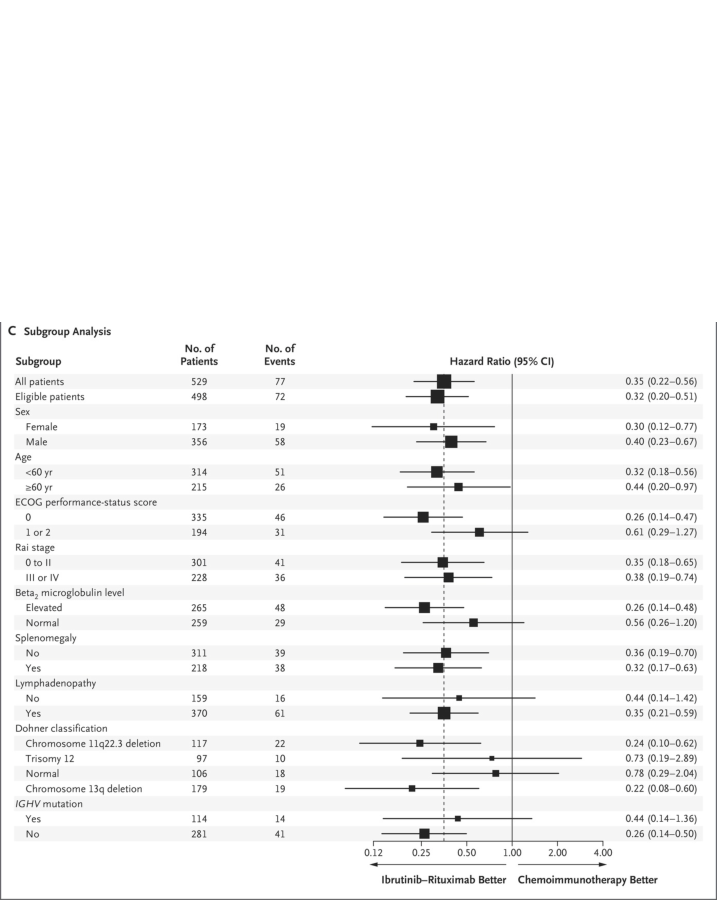
\includegraphics{../figures/shanafelt_subgroups.pdf}

\end{frame}

\begin{frame}{The wider debate about \(p\)-values}
\protect\hypertarget{the-wider-debate-about-p-values}{}

\(p\)-values

\begin{itemize}
\item
  do not indicate the size of an effect
\item
  nor do they indicate the likelihood of an effect
\end{itemize}

Fisher never intended `significant' to mean `statistically significant'

\begin{itemize}
\tightlist
\item
  Is `statistically significant' a meaningless term?
\end{itemize}

A true \(p < 0.05\) may not reduce the false positive rate enough

\end{frame}

\begin{frame}{False positive probability, p-value, power (Nat. Human
Behavior, Jan 2018)}
\protect\hypertarget{false-positive-probability-p-value-power-nat.-human-behavior-jan-2018-1}{}

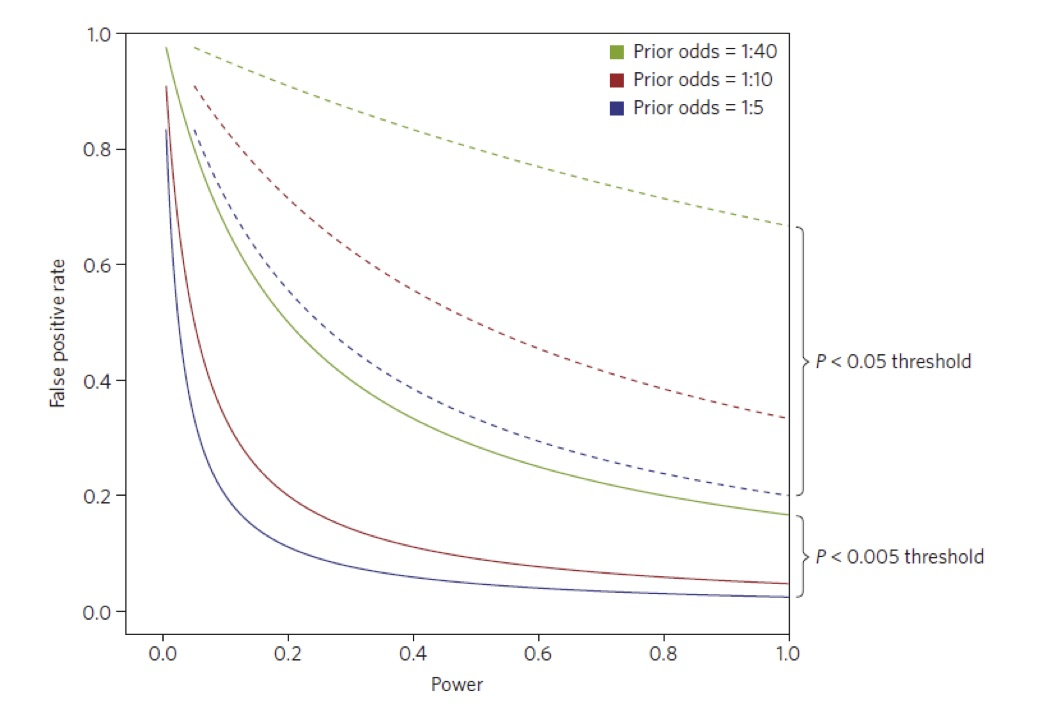
\includegraphics[width=1\textwidth,height=\textheight]{../figures/ppv_threshold.jpeg}

\end{frame}

\begin{frame}{The wider debate\ldots{}}
\protect\hypertarget{the-wider-debate}{}

From our editorial

\begin{quote}
The notion that a treatment is effective for a particular outcome if P<0.05 and ineffective if that threshold is not reached is a reductionist view of medicine that does not always reflect reality.
\end{quote}

But we need clearly articulated decision rules in evidence-based
medicine

\begin{itemize}
\tightlist
\item
  Reproducibility and Replicability in Science (2019)
  \url{http://nap.edu/25303}
\end{itemize}

\end{frame}

\begin{frame}{Also in the guidelines}
\protect\hypertarget{also-in-the-guidelines}{}

Principled analyses of studies with missing data

Acceptable to use unadjusted p-values for safety outcomes

Protocol and Statistical Analysis Plan (SAP) required for clinical
trials

Submit SAP for observational studies if it exists

Require model diagnostics for observational studies

Accompanying editorial gives references to methods for controlling error
rates with multiple tests

\end{frame}

\begin{frame}

Talk is available under mskcc\_2019-nejm at

\url{https://github.com/dave-harrington/talks}

\end{frame}

\begin{frame}{Some references}
\protect\hypertarget{some-references}{}

\small

Wasserstein RL, Schirm AL, Lazar NA. Moving to a world beyond
p\textless{}0.05. Am Stat. 2019;73:1-19.
\url{doi:10.1080/00031305.2019.1583913}

National Academies of Sciences, Engineering, and Medicine.
Reproducibility and replicability in science. Washington, DC: National
Academies Press, 2019. \url{http://nap.edu/25303}

Dmitrienko A, D'Agostino RB Sr.~Multiplicity considerations in clinical
trials. N Engl J Med 2018;378:2115-22.

Benjamin DJ, et al.~Redefine statistical significance. Nat Hum Behavior
2018;2:6-10. doi: 10.1038/s41562-017-0189-z

Ioannidis JPA. Retiring statistical significance would give bias a free
pass. Nature. 2019;567 (7749):461. \url{doi:10.1038/d41586-019-00969-2}

\end{frame}

\end{document}
